%********************************************************************************
% Title: Grand Challenge: Real-time Analysis of Social Networks
%		 Leveraging the Flink Framework
%
% Conference: ACM DEBS 2016
%
% Authors: Giacomo Marciani <giacomo.marciani@gmail.com>,
% 		   Marco Piu <pyumarco@gmail.com>,
%		   Michele Porretta <micheleporretta@gmail.com>,
%		   Matteo Nardelli <nardelli@ing.uniroma2.it>,
%		   Valeria Cardellini <cardellini@ing.uniroma2.it>
%
% Institution: Department of Civil Engineering and Computer Science Engineering,
% 			   University of Rome Tor Vergata, Italy
%
% Style: SIG Proceedings Alternate VERSION 2.8
%********************************************************************************

\documentclass{sig-alternate-05-2015}

\usepackage{graphicx}
\usepackage{epstopdf}
\usepackage{subfig}
\usepackage{bm}
\usepackage{url}

%% XXX: --- cancellare questa sezione ---
\usepackage[usenames,dvipsnames]{color}
\newcommand{\hlr}[1] {\emph{{\color{red}#1}}}
\newcommand{\hlb}[1] {\emph{{\color{blue}#1}}}
%% XXX: FINE --- cancellare questa sezione ---


%********************************************************************************
% Paper Size as US Letter
%********************************************************************************
\setlength{\paperheight}{11in}
\setlength{\paperwidth}{8.5in}
\usepackage[pass]{geometry}

%********************************************************************************
% Custom Rules
%********************************************************************************

\def\sharedaffiliation{%
\end{tabular}
\begin{tabular}{c}}

\newfont{\eaddfntresz}{phvr8t at 11pt}

\hyphenation{sched-uler par-a-digm adopt-ed evolv-ing th}

%********************************************************************************
% Avoid beaking after first/last line of a paragraph
%********************************************************************************

\clubpenalty=10000
\widowpenalty=10000

\begin{document}

%********************************************************************************
% Paper ACM Details
%********************************************************************************

\CopyrightYear{2016}
\setcopyright{rightsretained}
\conferenceinfo{DEBS '16}{June 20-24, 2016, Irvine, CA, USA}
\isbn{978-1-4503-4021-2/16/06}
\doi{http://dx.doi.org/10.1145/2933267.2933517}


%********************************************************************************
% Title and Authors
%********************************************************************************

\title{Grand Challenge: Real-time Analysis of Social Networks \\ Leveraging the Flink Framework}

\numberofauthors{5}
\author{
\alignauthor
	Giacomo Marciani\\
	\email{{\eaddfntresz giacomo.marciani@gmail.com}}
\alignauthor
	Marco Piu\\
	\email{pyumarco@gmail.com}
\alignauthor
	Michele Porretta\\
	\email{micheleporretta@gmail.com}
\and
\alignauthor
	Matteo Nardelli\\
	\email{nardelli@ing.uniroma2.it}
\alignauthor
	Valeria Cardellini\\
	\email{cardellini@ing.uniroma2.it}
\sharedaffiliation
	\affaddr{Department of Civil Engineering and Computer Science Engineering}  \\
	\affaddr{University of Rome Tor Vergata, Italy}
}

\maketitle

%********************************************************************************
% Content
%********************************************************************************

\begin{abstract}
	
In this paper, we present a solution to the DEBS 2016 Grand Challenge that leverages Apache Flink, an open source platform for distributed stream and batch processing. The challenge focuses on the real-time analysis of an evolving social-network graph, to (1) determine the posts that trigger the current most activity, and (2) identify large communities that are currently involved in a topic.  

We design the system architecture focusing on the exploitation of parallelism and memory efficiency so to enable an effective processing of high volume data streams on a distributed infrastructure.

Our solution to the first query relies on a distributed and fine-grain approach for updating the post scores and determining partial ranks, which are then merged into a single final rank. Furthermore, changes in the final rank are efficiently identified so to update the output only if needed.

The second query efficiently represents in-memory the evolving social graph and uses a customized Bron-Kerbosch algorithm to identify the largest communities active on a topic. We leverage on an in-memory caching system to keep the largest connected components which have been previously identified by the algorithm, thus saving computational time.

We run the experiments on a single node equipped with 4 cores, 8 GB of RAM and SSD with 900 IOPS. For a medium dataset size with 200k events, our system can process up to 2.5(?) kEvents/s with an average latency of 0.4(?) ms for the first query, and up to 2.8(?) kEvents/s with an average latency of 0.5(?) ms for the second query. 
		
\end{abstract}

%%%%%%%%%%%%%%%%%%%%%%%%%%%%%%%%%%%%%%%%%%%%%%%%%%%%%%%%%%%%%%%%%%%%%%%% 
% ACM Computing Classification System
%%%%%%%%%%%%%%%%%%%%%%%%%%%%%%%%%%%%%%%%%%%%%%%%%%%%%%%%%%%%%%%%%%%%%%%% 
% The code below should be generated by the tool at
% http://dl.acm.org/ccs.cfm
% Please copy and paste the code instead of the example below. 
%%
\begin{CCSXML}
<ccs2012>
<concept>
<concept_id>10002951.10002952.10002953.10010820.10003208</concept_id>
<concept_desc>Information systems~Data streams</concept_desc>
<concept_significance>500</concept_significance>
</concept>
%<concept>
%<concept_id>10003033.10003099.10003100</concept_id>
%<concept_desc>Networks~Cloud computing</concept_desc>
%<concept_significance>300</concept_significance>
%</concept>
</ccs2012>
\end{CCSXML}
%
\ccsdesc[500]{Information systems~Data streams}
%\ccsdesc[300]{Networks~Cloud computing}
%% End generated code
%%
%%  Use this command to print the description
\printccsdesc
%%%%%%%%%%%%%%%%%%%%%%%%%%%%%%%%%%%%%%%%%%%%%%%%%%%%%%%%%%%%%%%%%%%%%%%% 


% A category with the (minimum) three required fields
% \category{C.2.4}{Distributed Systems}{Distributed applications}
% \category{D.4.7}{Organization and Design}{Distributed systems}

\keywords{Social-network graphs,
Real-time data processing, Flink}
%Apache Flink, Redis}
\section{Introduction}
\label{sec:introduction}

The social network analysis (SNA) is a discipline that for years conveys the interest of the scientific community and industry. 
The identification of the components in a social graph that mostly stimulate the interaction between network nodes, is an activity that is gaining more and more strategic value within data-driven business models. 
The introduction of new computational paradigms and activating technologies has enabled the spread of this analysis in the everyday life: from the rankings proposed by the most common social networks, to the most cutting-edge scientific applications. 
The extraction of informational value from a social graph must often deal with algorithms, whose complexity requires the use of heuristics and a high degree of computational distribution.

The purpose of our work is to meet the Grand Challenge's requirements with an efficient, easily extendable measurable and tunable solution, which can run on a single node, but whose architecture is designed to be executed in a distributed environment. Willing to model the solution as a data stream processing application, we wanted to specifically experience the Flink framework \cite{Flink}, as it is highly innovative and relatively new on the $\lambda$-architecture landscape.

The rest of the paper is organized as follow. In Section \ref{sec:solution} we show the general architecture of our solution and the topology of the operators for the first and second query. In this section we also come into the design details of the system's core components. In Section \ref{sec:evaluation} we show the results obtained from experiments conducted on datasets which are variations of the one proposed in the challenge, that preserve the original event distribution. In Section \ref{sec:future-works} we anticipate future improvements planned for our solution, with a view to its implementation in a distributed environment.
\section{Grand Challenge Solution}
\label{sec:solution}

For the solution a number of data processing open source frameworks have been examined, including Apache Storm and Apache Spark Streaming. Eventually, our choice fell on Flink, an Apache Foundation top project which implements a $\lambda$-architecture. The architecture of our soultion exploits some of the Flink peculiar features, the most relevant being the possibility to have a feedback 
towards upstream operators. This characteristic can be very useful in optimizing stateful nodes using data from downstream operators. In the first query it is used to delete expired posts which cannot be among the top scorer anymore. In this way we can prevent a fast growth on memory consumption as well as having only tuples around the system that con actually affect the top score.
Having to deal with graphs, we also needed something to store the data structure and that would be accessible by all the operators in the system. We dealt with this problem using Redis (Jedis API), an in-memory key-value, NoSQL database. Its versatility permits to have various data types stored in main memory, avoiding the bottleneck given by mass storage I/O. In our solution we memorize in Redis the graph represented as an adjacency list.

\begin{figure}
	\centering
	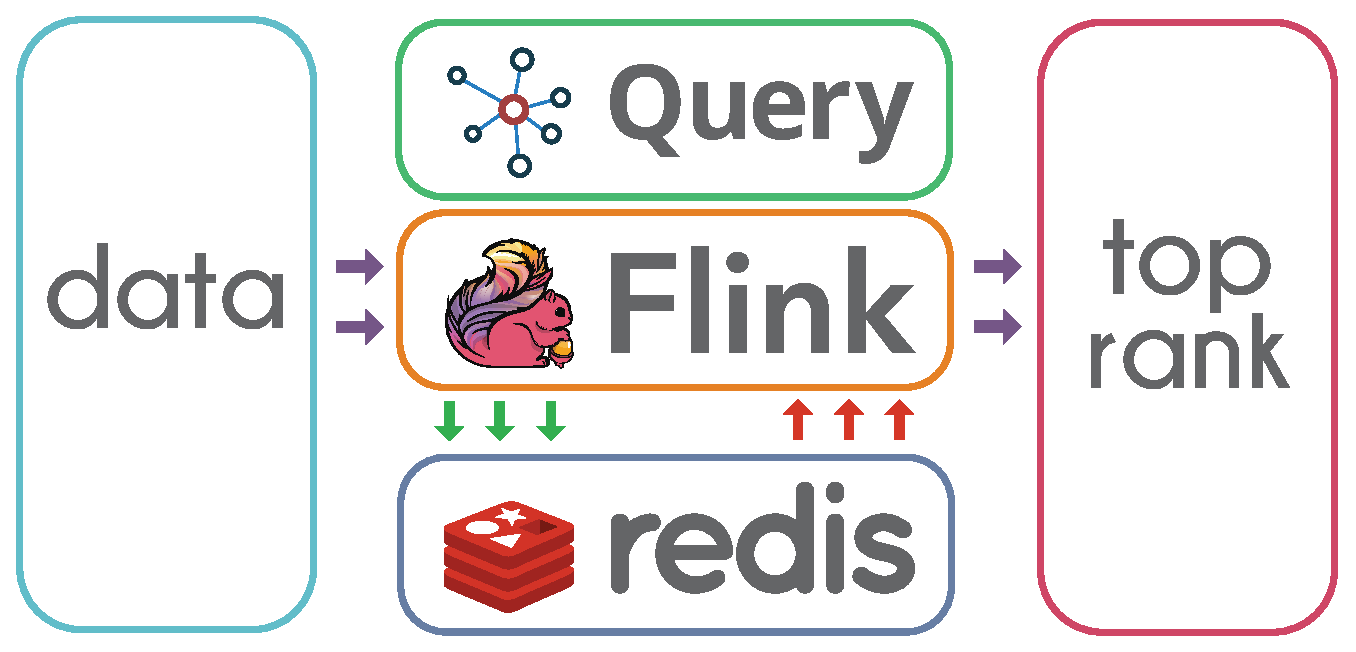
\includegraphics[width=\columnwidth]{fig/sostream-layered-architecture}
	\caption{The layered architecture}
	\label{fig:sostream-layered-architecture}
\end{figure}
\subsection{Query 1}
Lorem ipsum dolor sit amet, consectetur adipiscing elit, sed do eiusmod tempor incididunt ut labore et dolore magna aliqua.Ut enim ad minim veniam, quis nostrud exercitation ullamco laboris nisi ut aliquip ex ea commodo consequat. Duis aute irure dolor in reprehenderit in voluptate velit esse cillum dolore eu fugiat nulla pariatur. Excepteur sint occaecat cupidatat non proident, sunt in culpa qui officia deserunt mollit anim id est laborum.

Lorem ipsum dolor sit amet, consectetur adipiscing elit, sed do eiusmod tempor incididunt ut labore et dolore magna aliqua.Ut enim ad minim veniam, quis nostrud exercitation ullamco laboris nisi ut aliquip ex ea commodo consequat. Duis aute irure dolor in reprehenderit in voluptate velit esse cillum dolore eu fugiat nulla pariatur. Excepteur sint occaecat cupidatat non proident, sunt in culpa qui officia deserunt mollit anim id est laborum.

\begin{figure*}[t]
	\centering
	\includegraphics[width=0.8\textwidth]{img/q1}
	\caption{The topology of operators, Query 1.}
\end{figure*}

Lorem ipsum dolor sit amet, consectetur adipiscing elit, sed do eiusmod tempor incididunt ut labore et dolore magna aliqua.Ut enim ad minim veniam, quis nostrud exercitation ullamco laboris nisi ut aliquip ex ea commodo consequat. Duis aute irure dolor in reprehenderit in voluptate velit esse cillum dolore eu fugiat nulla pariatur. Excepteur sint occaecat cupidatat non proident, sunt in culpa qui officia deserunt mollit anim id est laborum.
\subsection{Query 2}
Lorem ipsum dolor sit amet, consectetur adipiscing elit, sed do eiusmod tempor incididunt ut labore et dolore magna aliqua.Ut enim ad minim veniam, quis nostrud exercitation ullamco laboris nisi ut aliquip ex ea commodo consequat. Duis aute irure dolor in reprehenderit in voluptate velit esse cillum dolore eu fugiat nulla pariatur. Excepteur sint occaecat cupidatat non proident, sunt in culpa qui officia deserunt mollit anim id est laborum.

Lorem ipsum dolor sit amet, consectetur adipiscing elit, sed do eiusmod tempor incididunt ut labore et dolore magna aliqua.Ut enim ad minim veniam, quis nostrud exercitation ullamco laboris nisi ut aliquip ex ea commodo consequat. Duis aute irure dolor in reprehenderit in voluptate velit esse cillum dolore eu fugiat nulla pariatur. Excepteur sint occaecat cupidatat non proident, sunt in culpa qui officia deserunt mollit anim id est laborum.

\begin{figure*}[t]
	\centering
	\includegraphics[width=0.8\textwidth]{img/q2}
	\caption{The topology of operators, Query2.}
\end{figure*}

Lorem ipsum dolor sit amet, consectetur adipiscing elit, sed do eiusmod tempor incididunt ut labore et dolore magna aliqua.Ut enim ad minim veniam, quis nostrud exercitation ullamco laboris nisi ut aliquip ex ea commodo consequat. Duis aute irure dolor in reprehenderit in voluptate velit esse cillum dolore eu fugiat nulla pariatur. Excepteur sint occaecat cupidatat non proident, sunt in culpa qui officia deserunt mollit anim id est laborum.
\section{Evaluation}
\label{sec:evaluation}

We evaluated the performance of our solution on a single Amazon EC2 instance running Debian 8.3 (Jessie), equipped with an Intel Xeon E5-2666 Haswell (2.6GHz, 4 cores and 25MB cache), 8 GB of RAM and SSD with 900 IOPS \cite{AWSEC2InstanceTypes}. 
Our solution is implemented in Java1.8 and relies on Apache Flink 1.0.0 \cite{Flink} and Redis 3.0.7 \cite{Redis}.

The experimental analysis aims to study (i) the overall latency, (ii) the average per tuple latency and (iii) the latency distribution on crucial operators. The times were measured using the analysis tools provided by the Flink framework.

Our solution aims to properly process the dataset proposed by the Grand Challenge in a timely-fashion. This dataset presents 55906573 events, distributed as follows:  44\% comments, 39\% likes, 15\% posts and 2\% friendships.

In the experimental phase, we considered portions of that dataset, preserving the original event distribution. In particular, we consider portions ranging from 0.1\% (55905 events) to 10\% (5590550 events) of the original dataset.

The experimental results show that:

\begin{enumerate}
	\item Workload balanced on operators: this makes our solution not affected by back-pressure in any portion of the stream and at no stage of computation.
	Workload balanced on cores.
	
	\item Physical memory is never close to saturation, thus avoiding overheads eventually caused by garbage collection and memory swapping.
	
	\item Presence of exponential complexity components.
	
	\item Heavy latency component due to the use of Redis in single node architecture.
\end{enumerate}
\section{Conclusions}
\label{sec:conclusions}

We have presented the design, implementation, and evaluation of our Flink-based solution to the DEBS 2016 Grand Challenge.
%
Despite its young age, Flink turned out to be a solid stream processing framework with some interesting features.   
%
An example is represented by the feedback stream, which has allowed us to minimize the wastage of memory, keeping its occupation low and steady, and 
to avoid back-pressure and performance degradation.
%
The experimental results, conducted in the reference environment, show that our solution can process up to 400 tuples/s with an average latency of 2.5~ms for the first query, and up to 370 tuples/s with an average latency of 2.7~ms for the second query, considering 50\% of the original Grand Challenge larger dataset.  

Leveraging the experience gathered to answer the Grand Challenge, we identify the following improvements as future work. 
%
We will exploit a finer-grained parallelism by enhancing the application components with more sophisticated data structures and operations, which enable concurrent and efficient updates.
%
To further reduce the average application latency, we will decouple the social events (e.g., post, comment, like) from their content (e.g., post message), so to reduce the streams transmission time.
%
Finally, we could make the feedback stream self-adaptive, so to properly handle the  back-pressure mechanism, even when posts expire with an unpredictable rate.

%********************************************************************************
% Bibliography
%********************************************************************************

\bibliographystyle{abbrv}
\bibliography{./ref/sostream}

\end{document}
